%Helper file which allows me compile the article without worrying about ABNT stuff

\documentclass[12pt]{article}
\usepackage[a4paper,top=25mm,bottom=25mm,width=150mm]{geometry}
\usepackage[brazilian]{babel}
\usepackage[backend=biber,style=authoryear,sorting=nyt]{biblatex}
\usepackage[T1]{fontenc}
\usepackage[utf8]{inputenc}
\addbibresource{refs.bib}
\usepackage{listings}
\usepackage{graphicx}
\lstset{language=Haskell,
  basicstyle=\ttfamily\scriptsize}

\newcommand{\figblocks}{
\begin{figure}
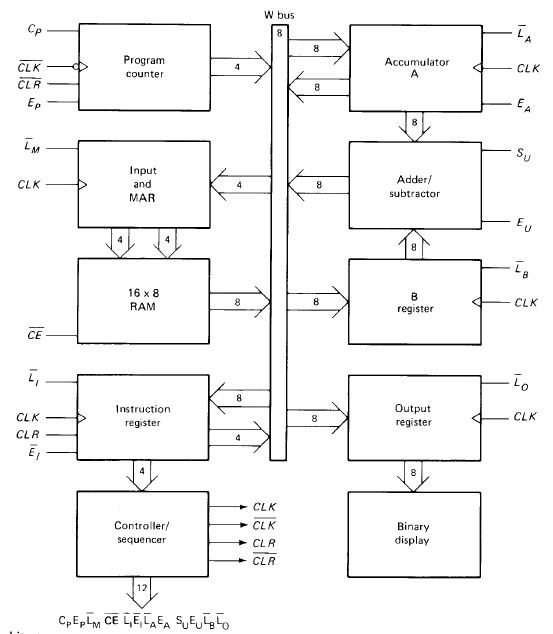
\includegraphics[width=0.6\linewidth]{figures/blocks.jpg}
\caption{Diagrama de blocos do processador SAP1. \cite{malvino}}
\label{f-blocks}
\end{figure}
}

\newcommand{\figblockmux}{
\begin{figure}
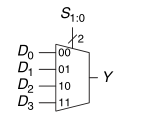
\includegraphics[width=0.5\linewidth]{figures/42-mux.png}
\caption{Bloco representando circuito multiplexador 4:2.}
\label{f-42mux}
\end{figure}
}

\newcommand{\fighmux}{
\begin{figure}
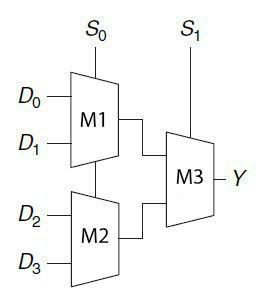
\includegraphics[width=0.5\linewidth]{figures/h-mux.jpg}
\caption{Diagrama de circuito multiplexador 4:2 construido hierarquicamente usando 3 multiplexadores 2:1.}
\label{f-hmux}
\end{figure}
}

\newcommand{\figcd}{
\begin{figure}
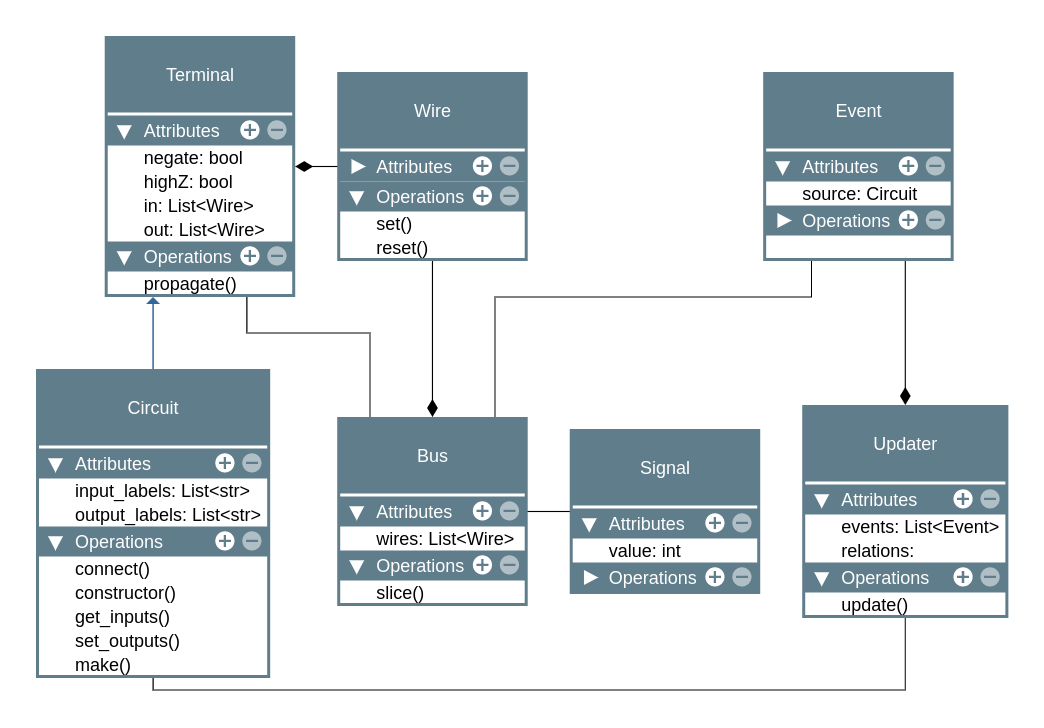
\includegraphics[width=\linewidth]{figures/class-diagrams.png}
\caption{Diagrama de classes para ferramenta.}
\label{f-cd}
\end{figure}
}

\newcommand{\logo}{

\includegraphics[width=0.3\textwidth]{figures/uninter-logo.png}\\
}

\newcommand{\parecer}{
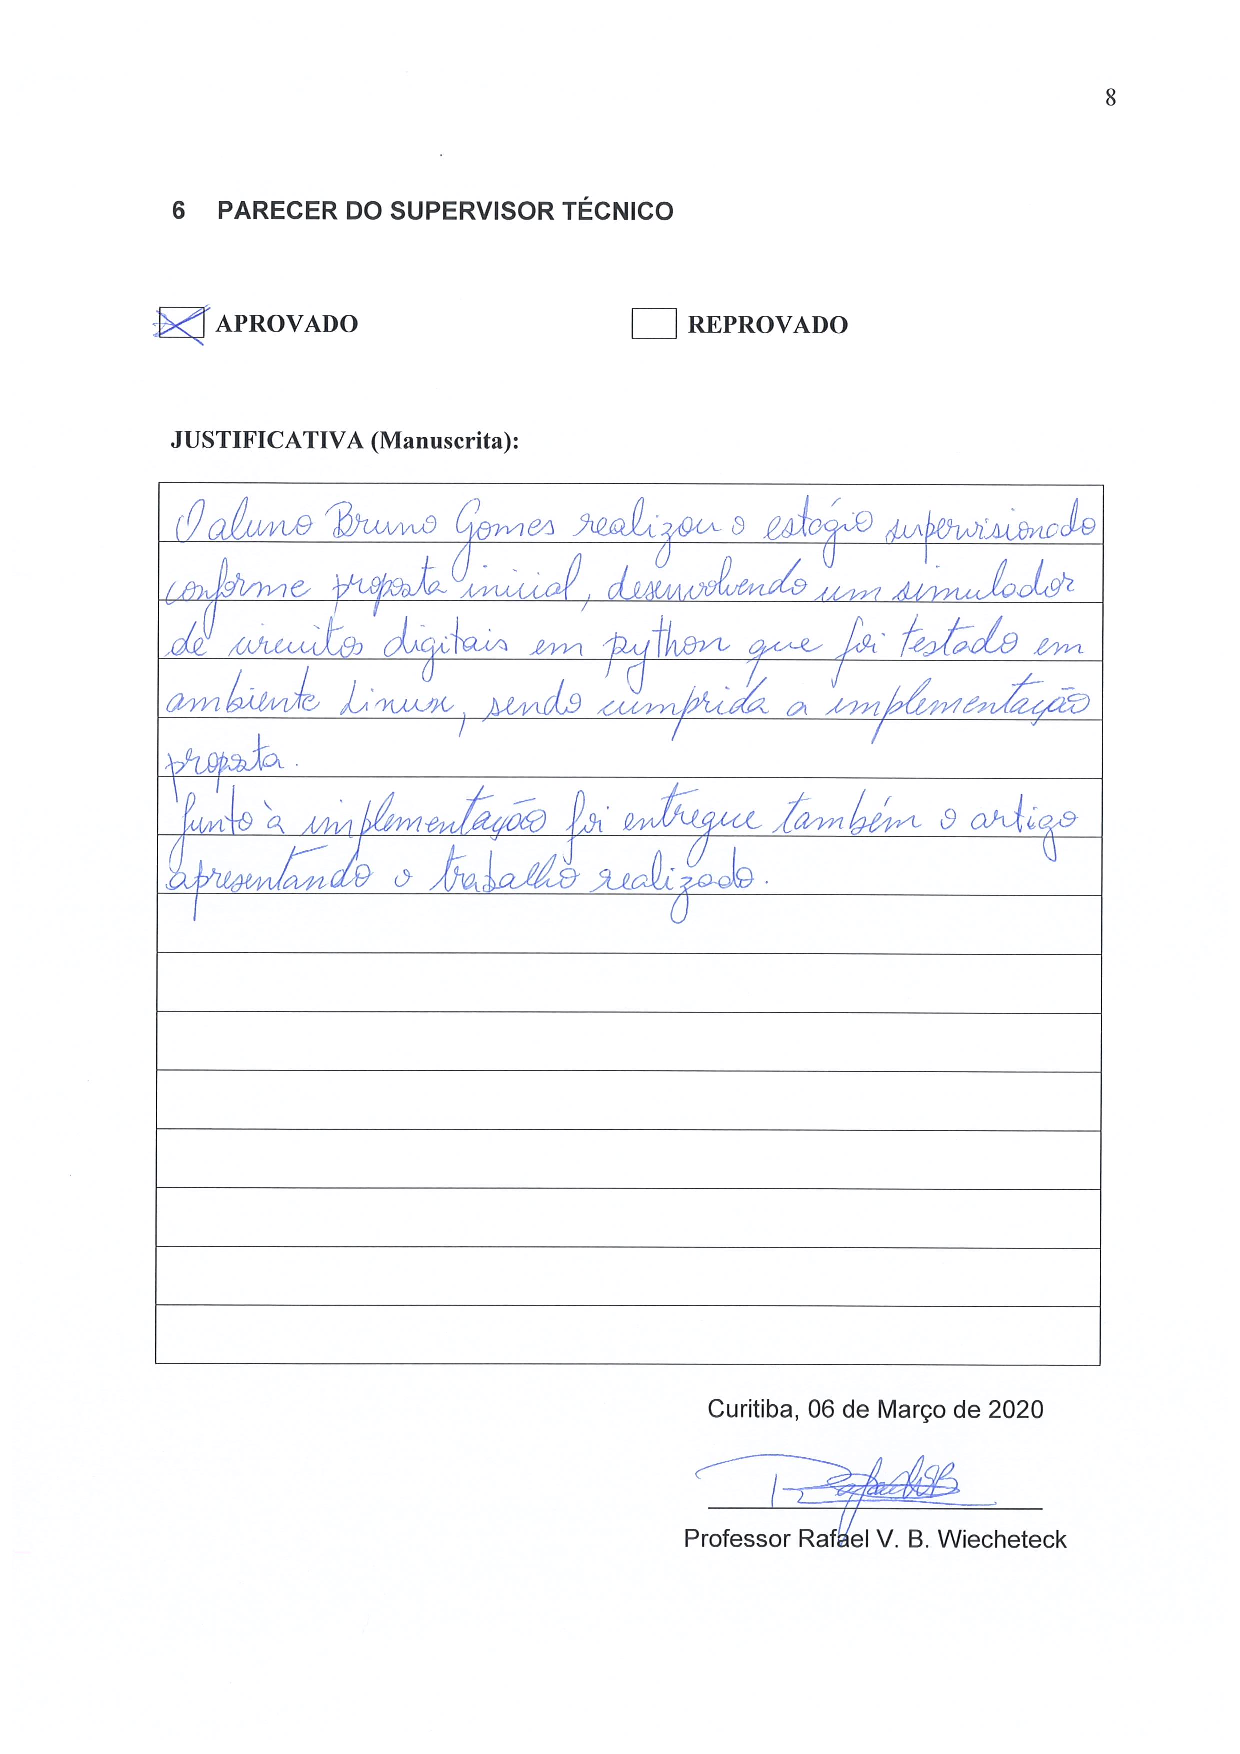
\includepdf[pages=-]{figures/parecer-tecnico.pdf}
}

\renewcommand{\cite}{\parencite}

\begin{document}
\title{Expressões regular em linguagem funcional: Módulo de busca usando expressões regulares implementado em Haskell}
\author{Bruno Gomes}
\date{\today}
\maketitle

\section{INTRODUÇÃO}
Qualquer estudante ou profissional que esteja envolvido no ambiente da tecnologia da informação certamente já teve contato com alguma espécie de linguagem de programação em algum ponto de sua jornada.
De acordo com uma pesquisa feita pelo StackOverflow, as 5 linguagens de programação mais usadas são: JavaScript, Python, Java, Linguagens de script (Bash, Powershell, Shell) e C\# \cite{stack-overflow}.

Embora essa lista de linguagens possa parecer como um conjunto heterogêneo de tecnologias, divergindo fortemente em convençoes e nichos de uso, todas essas linguagens fazem parte da família de linguagens conhecidas como imperativas.
Inquestionavelmente, as liguagens imperativas são muito importantes, pois as mesmas compõem a maioria do código sendo produzido diariamente, porém não são a única família de linguagens existentes.
Nesse trabalho será discutido o paradigma de programação funcional, uma alternativa ao paradigma imperativo que domina o mercado.

O foco desse trabalho será a criação de um módulo em Haskell para realizar buscas em textos usando expressões regulares.
Durante essa jornada serão feitas comparações entre algoritmos escritos de maneira imperativa e funcional, usando as linguagens Python e Haskell, respectivamente.
As expressões regulares partem da teoria da computação, mais especificamente da teoria das automatas.
Será definida a teoria as automatas, como elas são capazes de processar expressões regulares e finalemente será abordado a implementação de um módulo em Haskell para a busca em texto.

Embora o paradigma funcional seja muito menos disseminado, ele é de extrema importância e possuem um grande impacto fora de seu nicho. as descobertas e inovações 
Diferentes inovações e descobertas no paradgima funcional, de certo modo infecta as linguagens imperativas.
Como exemplo disso temos que a partir da versão 8 do Java, foram introduzidas interfaces funcionais e \emph{lambda expressions}, conceitos esses que surgiram a programação funcional \cite{java8}.

Em conclusão, embora as linguagem funcionais sejam muito menos comum, elas definitivamente deixaram e continuam deixando marcas nos gigantes da programação.
Elas transcendem seu pequeno nicho de usuários e afetam a grande maioria das pessoas que produzem código regularmente, mesmo que muitos não tenham ciência disso.
Sendo assim, esse trabalho tem como objetivo introduzir o paradigma funcional, através da linguagem Haskell, comparando os dois paradigmas e discutindo a maneira funcional de resolver certos problemas computacionais.

\section{EXPRESSÕES REGULARES E PROGRAMAÇÃO FUNCIONAL}
Como foi abordado na introdução, esse trabalho une dois temas: expressões regulares e programação funcional.
Esses temas serão, primeiramente, discutidos separadamente, e em seguida será feito uma previa de como será feita a construção do motor de processamento de expressões regulares.

\subsection{Introdução as expressões regulares}

Expressões regulares, tambem conhecidas como \emph{regex} (da junção do nome em inglês, \emph{regular expression}) são utilizadas para realizar buscas complexas sobre strings.
Para Cox,
"expressões regulares são uma notação que descreve um conjunto de strings.
Quando alguma string está no conjunto associado à expressão regular, pode-se dizer que essa expressão regular corresponde a esse string." \cite{cox}.

As regexes são utilizadas frequentemente, tanto para extrair informações que seguem um padrão ou para realizar buscas mais flexíveis ou parciais.
Como exemplo, suponha o problema de extrair todas os strings que correspondem a um horario em um texto.
A escrita de um horario segue uma estrutura padrão, HH:MM:SS onde HH delimita as horas, MM delimita os minutos e SS delimita os segundos.
Sem ter que construir todas as possíveis combinações de horas que seguem esse formato, uma simples varredura de texto é incapaz de extrair essa informação.
Esse problema pode ser resolvido tranquilamente usando regexes.

Uma expressão regular que realiza esta busca é,
\begin{equation}
  [0-9]\{2\}:[0-9]\{2\}:[0-9]\{2\} .
\end{equation}

Em palavras, os símbolos [0-9] representa qualquer carácter numerico entre 0 e 9.
De maneira geral os símbolos [] representam um conunto de caracteres \cite{python-re}.
O token \{2\} indica uma repetição, sendo equivalente à regex [0-9][0-9], ou seja dois carácteres numericos.
Os simbolos \{\} são usados para representar repetição \cite{python-re}.
O caractere ":" é interpretado de maneira literal.
Fazendo a união, a regex acima equivale a qualquer string que tenha o formato DD:DD:DD onde D indica qualquer digito de 0-9.
Podemos ver que esse formato é exatamente o formato definido anteriormente.

É importante ressaltar que existem inumeras variações e implementações de regexes, onde existem diferentes meta-caracteres para descrever operações.
Em \cite{mastering}, o autor discute as diferenças em regex entre as linguagens: PHP, .NET, Java e Perl.
Na documentação oficial da linguagem Python \cite{python-re} é dito que o dialeto usado é basedo nas expressões regulares da linguagem Perl com alguns adicionais.
Usuários UNIX também estão familiarizados com os \emph{wildcards} presentes nos shells, uma forma de regex.
Em resumo, existem diversos dialetos porém o objetivo das regexes não se altera, buscar por padrões.
A regex acima e todas as regexes subsequentes nesse texto serão escritos no dialeto da linguagem Perl. 

\subsection{Programação Funcional}

Essa seção aborda programação funcional e suas caracteristicas de maneira resumida.
Há muito a se falar sobre esse assunto pois ele é extensso e tem uma longa história.
Para abordar a programação funcional será tomado um foco que toma como base a computação.

De maneira geral, programas de computadores existem para resolver problemas computacionais.
Segundo \cite{matrix} um problema computacional é
" [...] uma especificação de entrada-saída que um procedimento tenha que satisfazer."
e um procedimento é
"[...] uma descrição precisa de uma computação; ele aceita entradas (chamadas de argumentos) e produz uma saída (chamado de valor de retorno).".
Ou seja, independente do paradigma utilizado para resolver o problema (funcional ou imperativa), ambos são capazes de definir um procedimento para um problema computacional, a grande diferença está em como esse procedimento é definido.

Segundo \cite{Bird},
\begin{quotation}
"Programção funcional é: um método para construção de programas que enfatiza funções e suas aplicações ao invéz de commandos e suas execuções; programação funcional faz uso de notações matemática simples que permite que problemas sejam descritos de maneira clara e concisa. [...]".
\end{quotation}
A programação imperativa foca em passos para resolver um problema, cada passo desse pode ser traduzido de maneira rasoavelmente direta em instruções de uma CPU.
Isso faz com que o procedimeto escrito imperativemente reflita muito mais a máquina do que ao homem.
O paradigma funcional tira o foco nos passos individuais para solucionar o problema e enfatiza uma estrutura para resolver o problema.

Em seguida serão abordados aspectos mais técnicos da programação funcional.

\subsubsection{Funções para resolver problemas}

Como visto anteriormente, a programação funcional propõe que problemas computacionais sejam resolvidos de maneira mais declarativa.
O foco muda de "quais passos é preciso para resolver esse problema" para "quais transformações aplicar nas minhas entradas para produzir a saída".

Para exemplificar essa idea considere o seguinte problema.
Dado uma lista de nomes, com nome, nome do meio e sobrenomes, crie uma lista com todas as combinações de primeiro nome e ultímo nome, ignorando nomes do meio e aonde as combinações cuja soma do primeiro e ultimo nome não exceda 15 caracteres (incluindo o espaço).
Para isso, ao invez de analisar os passos para processar esses dados, uma boa ideia é pensar em como manipular os dados para se obter o resultado desejado.
Para esse problema, sugere-se a seguinte solução:

\begin{enumerate}
\item{Separar cada nome da lista de nomes nos espaços e armazenar os nomes uma lista.}
\item{Filtrar listas que só possuem um elemento (somente um nome).}
\item{Filtrar listas e remover nomes do meio.}
\item{Criar uma lista de nomes e uma lista sobrenomes.}
\item{Realizar o produto cartesiano sobre essa lista e gerar uma lista de tuplas.}
\item{Tranformar tuplas em strings fazendo a concatenação do primeiro nome e do sobrenome.}
\end{enumerate}

Percebe-se que cada passo acima realiza uma única ação, sendo ela simples e clara e é interessante modelar cada um desses passos como uma função.
Na linguagem Haskell o tipos dos argumentos e do retorno de uma função é dado pela notação nomeDaFuncao :: arg1 -> arg2 -> ... -> retorno, onde arg1 e arg2 definem os tipos dos argumentos \cite{lipovaca}.
Para identificar listas em Haskell é usado o símbolo [], ou seja [Char] indica uma lista de caracteres e tuplas são indicatas com () onde (String, String) indica uma tupla com dois elementos, ambos strings.
Podemos agora reescrever o problema acima definindo todas as funções que serão utilizadas.

Primeiramente definiremos o problema enunciado como uma função usando a notação introduzida.
O problema inicial é a função $combinarNomes :: [String] -> [String]$ , ou seja uma função que recebe uma lista de Strings e retorna uma lista de Strings.
Em seguida, iremos declarar as funções que representam cada passo acima.

\begin{enumerate}
\item{separarNomes :: [String] -> [[String]]}
\item{tirarIncompleto :: [[String]] -> [[String]]}
\item{removerSobrenomes :: [[String]] -> [[String]]}
\item{gerarNomesESobrenomes :: [[String]] -> ([String], [String])}
\item{gerarCombinacoes :: ([String], [String]) -> [(String, String)]}
\item{concatenarNomes :: [(String, String)] -> [String]}
\end{enumerate}

Segundo \cite{lipovaca} a assinatura de uma função em Haskell combinado com um nome descritivo diz muito sobre a função e de fato, dados os nomes e sua assinatura, pode-se facilmente deduzir o que cada função está fazendo.

O objetivo dessa seção foi dar um exemplo alto nível de como é resolvido um problema de maneira funcional.

\subsection{Automatas e expressões regulares}

Como visto, as expressões regulares representam uma maneira conveniente de descrever conjutos de string.
Embora conveniente, a maneira na qual as expressões regulares foram introduzidas não permite uma tradução direta delas para um ambiente computacional.
Essa seção faz a ligação entre esses objetos teóricos e uma descrição matématica das mesmas.

\subsubsection{Definição de uma automata}

Segundo \cite{comp}, as automatas modelam um computador com uma quantidade minúscula de memória.
A ideia central de uma automata é representar uma estrutura computacional a partir de um conjunto de estados e entradas.

Os estados da automata constitui um conjunto denominado de $Q$, o conjunto de estados.
Dentre esses estados existe um único estado inicial da automata chamado de $q_o \in Q$.
Automatas recebem entradas a partir de simbolos, o conjuto de todos os símbolos reconhecidos por uma automata define um conjunto $\Sigma$ chamado de alfabeto da automata.
Os estados da automata podem ou não estar conectados, quando existe uma conexão entre dois estados essa conexão é representada por um simbolo $\alpha \in \Sigma$.
As transições entre estados de uma automata é representado por uma função $\delta$ onde $\delta : Q \times \Sigma \mapsto Q$, ou seja $\delta$ recebe dois argumentos, um estado e um símbolo e mapeia esse par a um estado.
Finalmente, a automata possui um conjunto de estados de aceitação $F$, onde $F \in Q$, caso a automata termine sua execução em um estado $q \in F$, o string de entrada foi aceito pela automata.
Formalmente, então, uma automata é uma tupla com 5 elementos $(Q, \Sigma, \delta, q_o, F)$ \cite{comp}.

A partir da descrição formal de uma automata, podemos definir uma rotina de computação.
De maneira breve, o objetivo dessa rotina é verificar que após processar o string de entrada a automata se encontra em um estado de aceitação.

Como foi visto, uma automata pode receber um conjunto de entradas que definem seu alfabeto $\Sigma$.
Deseja-se definir um procedimento onde dado um string de entrada e uma automata no seu estado inicial, retorne o estado final após processar a entrada.
Esse procedimento é definido como dado uma entrada $w=w_1w_2...w_n \mid w_i \in \Sigma$ e uma automata $M$ no seu estado inicial, será retornado um estado $q \in Q$.
Caso o estado final seja um estado de aceitação ($q \in F$), é dito que $M$ aceita $w$ \cite{comp}.
Formalmente, segundo \cite{comp} $M$ aceita $w = w_1w_2...w_n$ se: existe uma sequencia de estados $r_0, r_1, ... r_n \in Q$ se $r_0 = q_0$; $\delta(r_i, w_{i+1}) = r_{i+1},$ para $i = 0, ..., n-1$; $r_n \in F$.

O ponto chave desse discussão é apresentado por \cite{comp}, onde foi provado que é possível construir uma automata para qualquer regex.
Sendo assim, é possível definir padrões de busca usando uma expressão regular, converter essa expressão regulara para uma automata e usar essa automata para realizar a busca pelo padrão em um string.

\subsection{METODOLOGIA}

Como explicado na introdução, o foco destre trabalho é demonstrar alguns  elementos da programação funcional.
Para isso, foi escolhido o problema de implementar um módulo de busca de strings usando expressões regulares.
Será escolhido trechos de código especialmente interessante do módulo escrito que serão explciados a fundo.

Foi visto que uma expressão regular pode ser convertida em uma automata equivalente.
Sendo assim, o problema possui duas tarefas: criar submódulo para converter uma regex em uma automata e implementar um submódulo que permita criar e operar uma automata.
Serão definidas as arquiteturas de cada submódulo tal como o encadeamento de funções que serão chamadas para resolver cada problema, análogo ao que foi feito anteriormente.
Será explicado, de maneira alto nível, o que cada função faz baseada em suas entradas e saídas.
Isso irá motivar a introdução de tipos de dados únicos a programação funcional.

Além dessa inspeção de "caixa preta" das funções, os pontos principais do módulo será explicado em detalhe, o que permitirá aa análise de conceitos importantes no paradigma funcional.
Será feita uma comparação entre trechos escrito de maneira funcional e imperativa.
Essa comparação tem dois objetivos: introduzir conceitos referentes a linguagem funcional e identificar em quais situações um código funcional é mais simples, ou mais complexo, que o seu equivalente de maneira imperativa.
Para introduzir os conceitos do paradigma funcional, o código irá ser projetado tal que demonstre as diferentes ferramentas que compõe a caixa de ferramentas de um programador funcional.
As ferramentas simples abordarão conceitos comos imutalidade e recursão e as ferramentas mais complexas irão introduzir abstrações muito perculiares da programação funcional tal como \emph{Functors} e \emph{Applicative Functors}.
A metodologia escolhida tem como objetivo ser transparente quanto aos lados bons e ruins da programação funcional e também auxiliar a associação do paradigma imperativo ao funcional.
Dessa forma, um leitor familiar com programação imperativa poderá entender como um problema resolvido de maneira imperativa pode ser traduzido para um algoritimo funcional.

Em conclusão, o trabalho irá resolver o problema de criar um módulo de procura em texto usando expressões regulares.
O problema será quebrado em funções, exemplificando como resolver um problema a partir de funções ao invez de passos.
O código fonte do módulo criado será usado para introduzir conceitos sobre o paradigma funcional e familiarizar o leitor com algumas ferramentas.
Ao mesmo tempo, trechos de códigos funcionais serão comparados com seu equivalente escrito em uma linguagem imperativa, o que permitira associar conceitos imperativos a funcionais e expor os pontos fortes e fracos desse paradigma.


\subsection{CONCLUSÃO}
Durante o projeto de estagio foi construído uma ferramenta em Python para simulação de circuitos digitais.
Essa ferramenta faz uso do paradigma de programação orientada a objetos para descrever um circuito.
Sendo assim, a implementação de um circuito é feita a partir de classes codificadas pelos usuários.
Essa metodologia garante circuitos modulares e regulares pois faz uso do conceito de herança para garantir uma interface consistente entre circuitos.

A ferramenta desenvolvida foi utilizada para construir um processador SAP1, uma arquitetura didática.
A ferramenta se mostrou capaz de simular o processador corretamente, porém foi notável um problema de performance.
Esse problema está relacionado a metodologia hierárquica empregada pela ferramenta.
Possíveis soluções para o problema foram abordadas na seção de analise.

O intuito da ferramenta é criar uma descrição simplificada de circuitos para que estudantes possam construir circuitos de maneira simples com o objetivo de facilitar ao processo de aprendizado.
Espera-se que um estudante possa construir um processador, a partir de uma bibliografia, sem que isso seja uma tarefa complexa e longa.
Sendo assim, essa ferramenta tenta substituir, até certo ponto, a construção de um processador em uma breadboard (processo longo) ou em uma linguagem HDL (processo complexo).

\section{CRONOGRAMA REALIZADO}
\section{CRONOGRAMA REALIZADO}
\section{CRONOGRAMA REALIZADO}
\input{tables/cronograma}



\printbibliography
\end{document}
